\begin{figure}[htb]
    \centering
    \begin{minipage}{.48\textwidth}
      \centering
      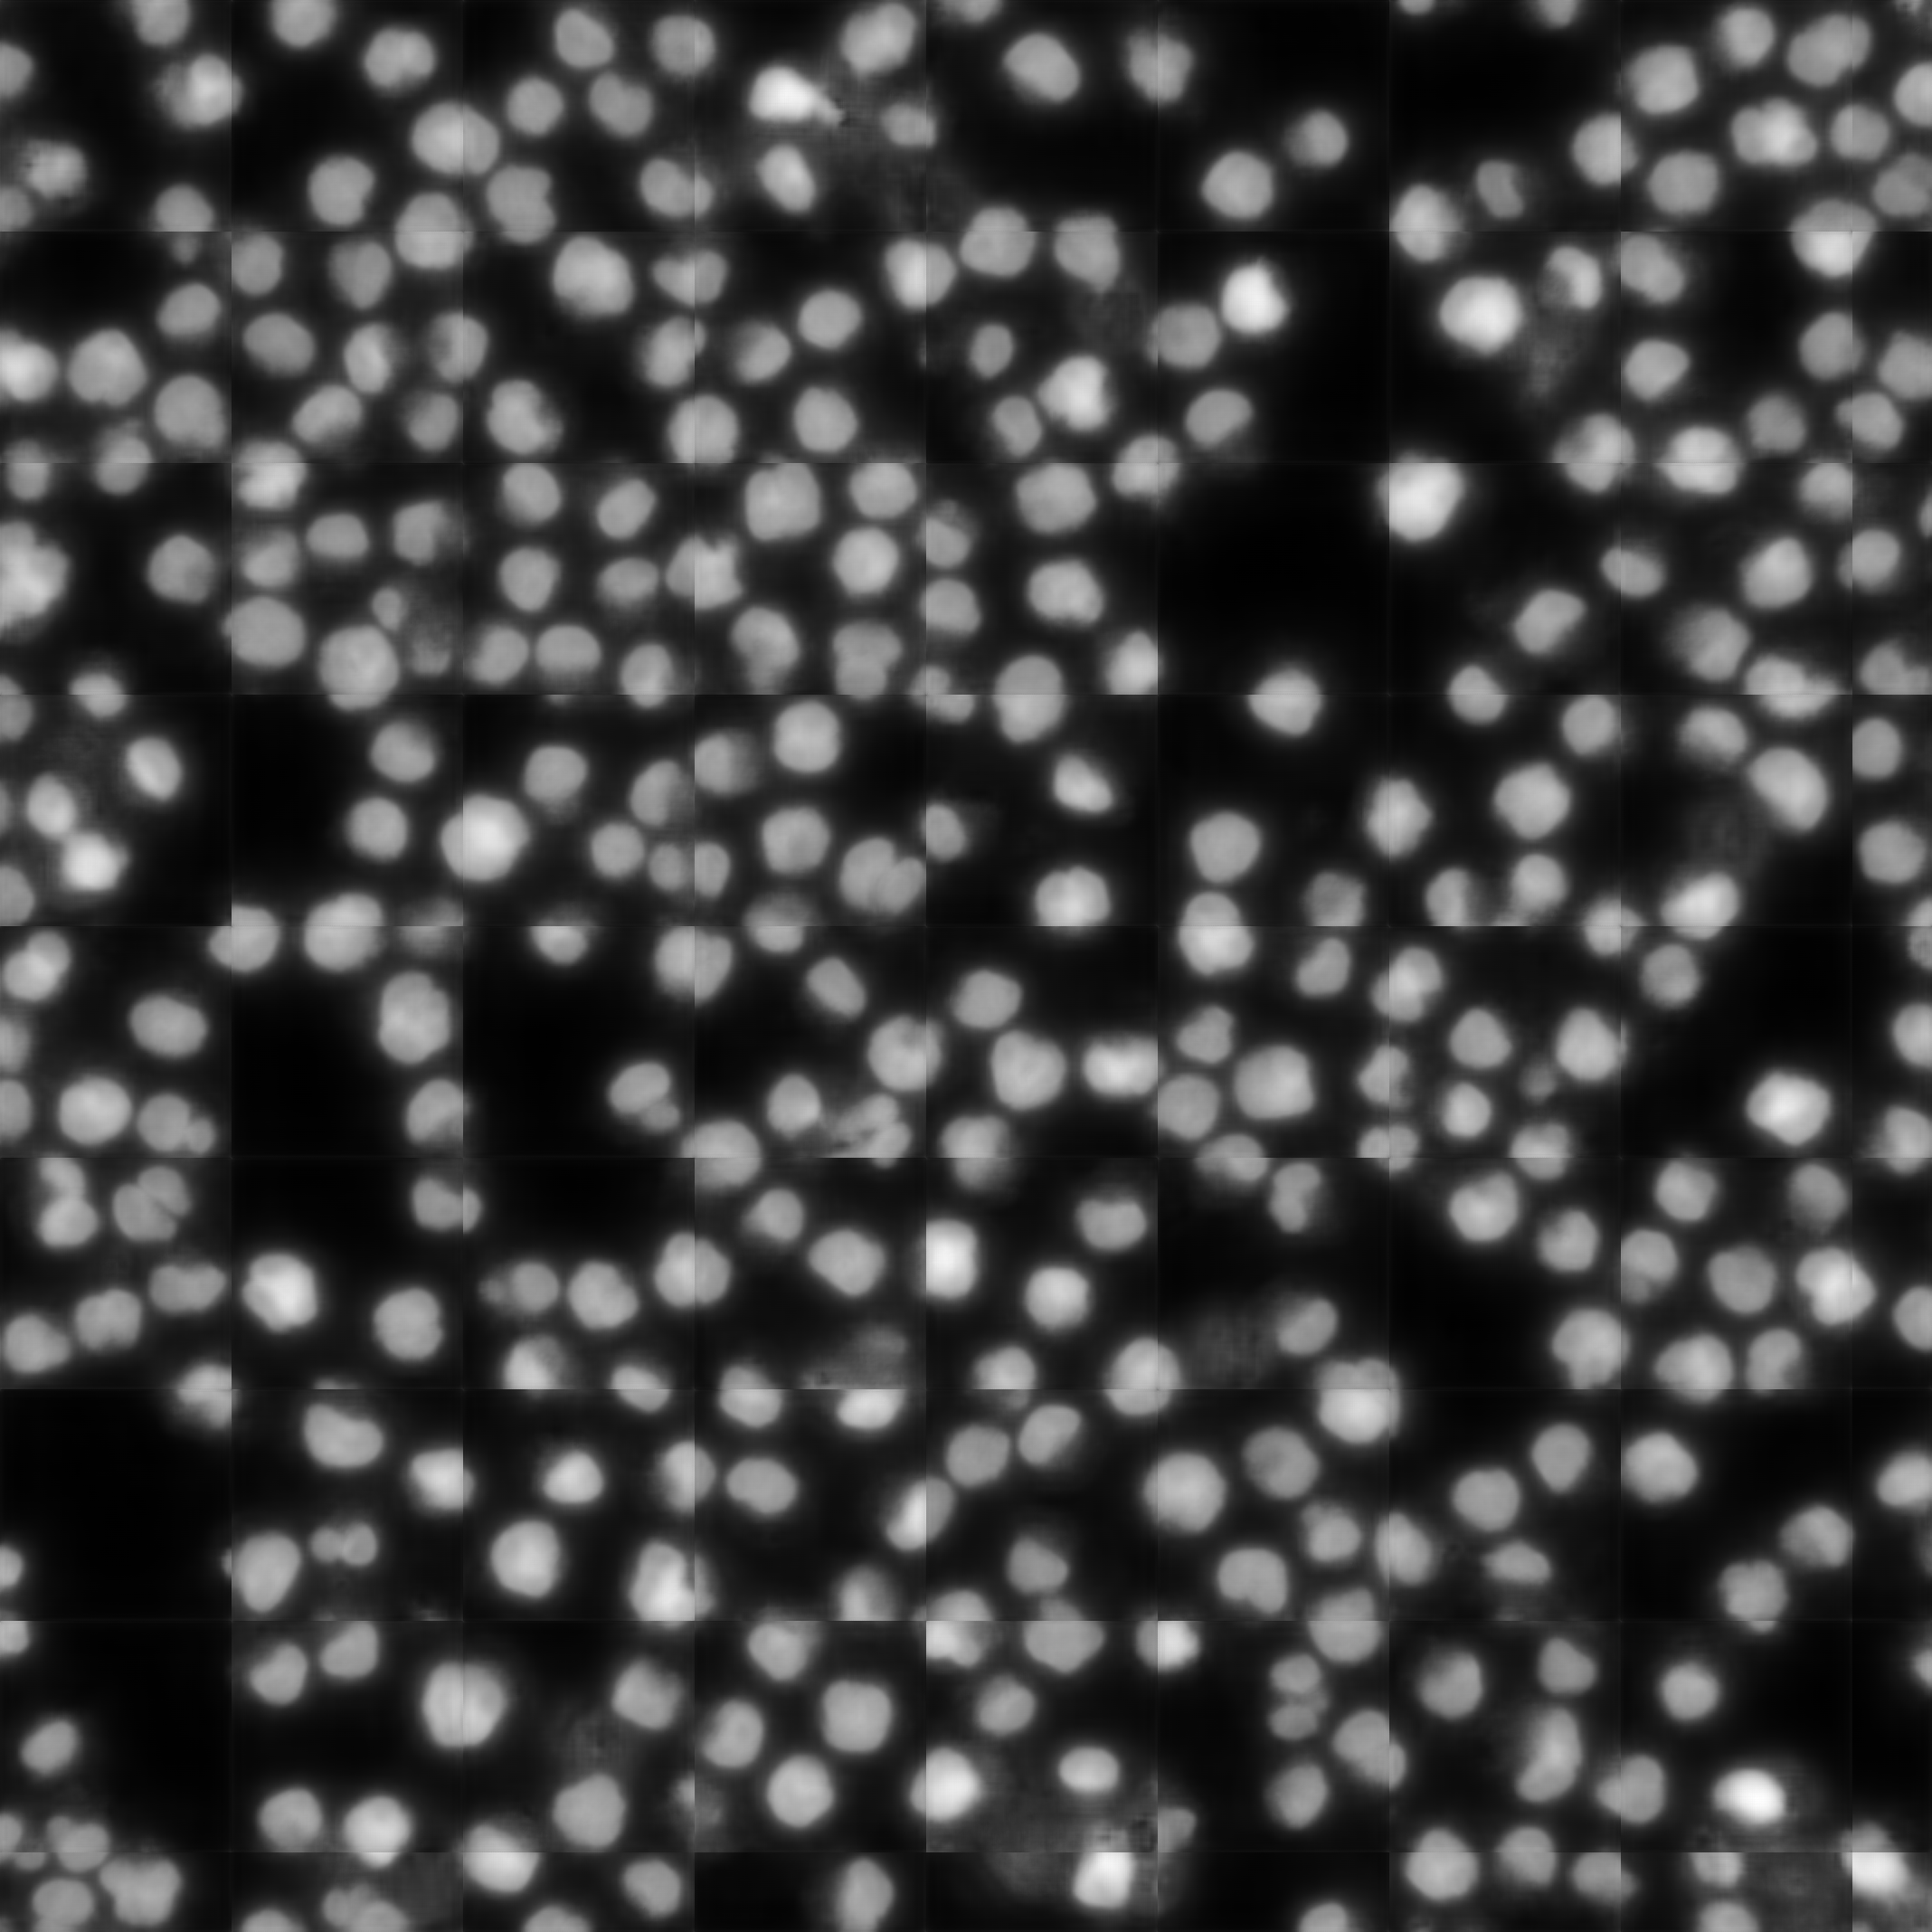
\includegraphics[width=\linewidth]{bilder/crops_combination/prediction_border_0.png}
      \caption{No overlap}
      \label{fig:crops_combination_0}
    \end{minipage}%
    \vspace{1cm}
    \begin{minipage}{.48\textwidth}
      \centering
      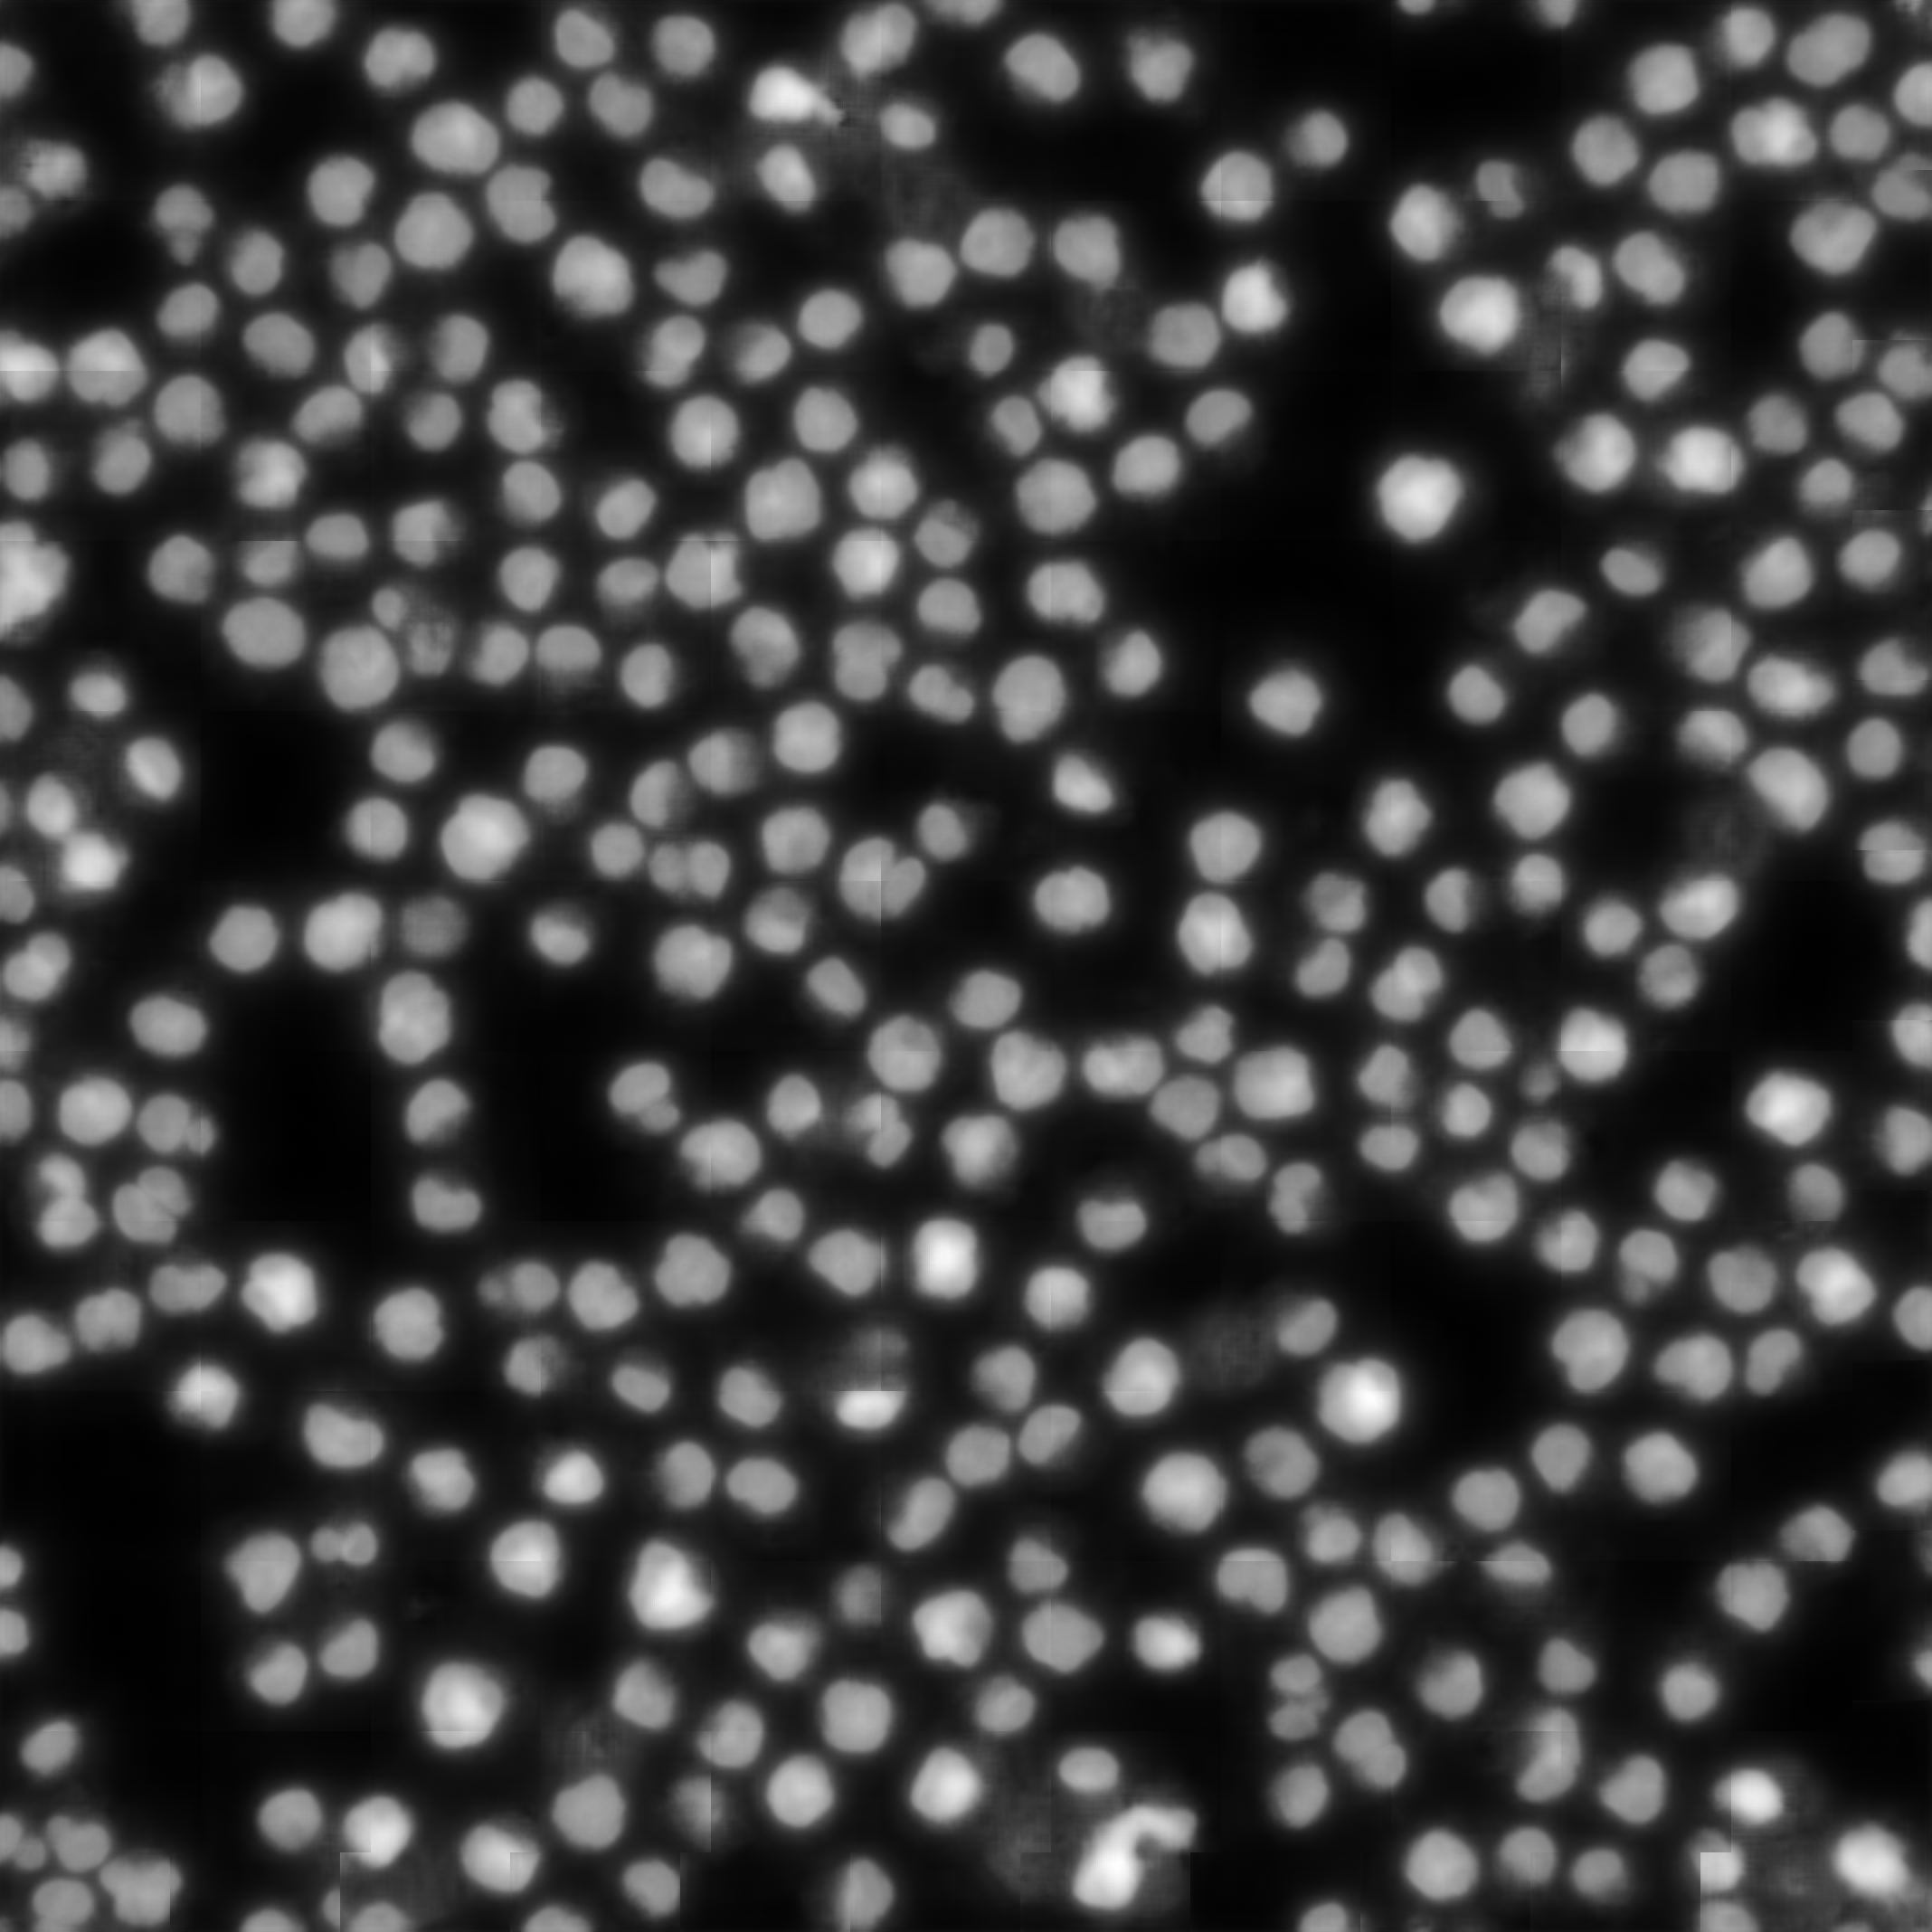
\includegraphics[width=\linewidth]{bilder/crops_combination/prediction_border_34.png}
      \caption{30 pixels overlap}
      \label{fig:crops_combination_34}
    \end{minipage}
\end{figure}


Improve this plot by showing the visible border explicitly, example of how it can influence a further segmentation perhaps?